\documentclass[10pt,a4paper]{amsart}
\usepackage[margin=19mm]{geometry}
\usepackage{amsmath,amssymb,mathtools}
\usepackage[scr=rsfs,cal=euler]{mathalfa}
\usepackage{xfrac}
\usepackage[unicode,hidelinks,bookmarks=false]{hyperref}
\newcommand{\ie}{i.e.\ }
\newcommand{\cf}{cf.\ }
\newcommand{\resp}{respectively\ }
\newcommand{\Subsection}{\subsection}
\providecommand{\nobreakdash}{\nobreak\hbox{-}}
\setlength{\emergencystretch}{2em}
\multlinegap0pt
\usepackage{tikz}
\usepackage[shortlabels]{enumitem}
\usepackage{float}
\usepackage{csquotes}
\newtheorem{lemma}{Lemma}
\newtheorem{proposition}{Proposition}
\usepackage{cleveref}
\crefname{lemma}{Lemma}{Lemmas}
\crefname{proposition}{Proposition}{Propositions}
\title{Bounded core partitions and Borel--Weil--Bott}
\author{Fern Gossow, Andrew Huchala}
\date{Source: arXiv:2510.17239v2 (CC BY 4.0)}
\begin{document}
\maketitle

\noindent\emph{Source and licence.} Bounded core partitions and Borel--Weil--Bott. Version arXiv:2510.17239v2 (CC BY 4.0), distributed by arXiv under the Creative Commons Attribution 4.0 International licence, http://creativecommons.org/licenses/by/4.0/, as recorded in the arXiv licence metadata for this exact version and shown on the abstract page https://arxiv.org/abs/2510.17239v2. Full licence notice: \texttt{licenses/arxiv-2510.17239-CC-BY-4.0.txt}.\par\smallskip

\noindent\textit{Editorial scope.} Counted unit: the article's proposition proposition (source0.tex lines 1172--1175). The article's complete original proof of it is delivered with it (source0.tex lines 1176--1197, one \texttt{proof} environment of 22 lines). No mathematics is written, repaired or re-derived: the statement and the proof are the article's own lines, in the article's own notation, and no retained line is substituted or re-flowed.  Retained uncounted as the source-local context the proof needs: lines 903--911; lines 1139--1146.  Nothing was omitted from any retained span, so the package carries no omission record.  No retained line contains a citation, so the wrapper carries no bibliography and no bibliography entry.  The retained lines contain the article's own diagram code, which the wrapper typesets with the standard tikz packages; no image file is delivered and the package declares no asset dependency.  Editorial formatting only, in addition: an AMS \texttt{amsart} preamble that restates the article's own declarations and macros used by the retained lines, namely the environments \texttt{lemma}, \texttt{proposition} on separate counters, together with the standard packages those lines need.  The retained environments print in this document as Lemma 1, Proposition 1 in order of appearance, whereas the article prints the same items with the numbering of its own full document.  The complete native source of the article as distributed in the arXiv e-print for this exact version is bundled unchanged as \texttt{sources/187398/source0.tex}.
\begin{lemma}\label{lem:nakano}
For a plane partition $P$, choose $k,n,j,i$ such that
\begin{itemize}
\item $k$ is the sum of the first column of $P$,
\item $n-k$ is the sum of the first row of $P$,
\item $i=|\Delta P|$ and $j=|\Delta P|+|P|$.
\end{itemize}
Then $i+j\leq k(n-k)$.
\end{lemma}

We now state improved versions of these bounds. These hold under the assumption that $t>0$. Note that the inequalities are reversed, since these are necessary conditions for the existence of Snow partitions.
\begin{enumerate}[label=(P\arabic*)]
\item $i\leq\dfrac{k-1}{k+1}j$, \medskip\label{eq:p1}
\item $i+j\leq N$, \medskip \label{eq:p2}
\item $j\leq\dfrac{1}{2}k(n-k+t-1)$, \medskip \label{eq:p3}
\item $j-i\geq t$ if $i>0$, \medskip \label{eq:p4}
\item $i\leq\dfrac{k-1}{2k}N$. \medskip \label{eq:p5}
\end{enumerate}

\begin{proposition}
Every $(t-1,t-1)$-bounded plane partition $P$ satisfies \emph{\ref{eq:p1}}, \emph{\ref{eq:p2}}, \emph{\ref{eq:p3}} and \emph{\ref{eq:p5}}, with $k,n,j,i$ as in \Cref{lem:nakano}. Moreover, we have
\[i\leq\frac{\sqrt{N}(\sqrt{N}-1)}{2}.\]
\end{proposition}

\begin{proof}
\Cref{lem:nakano} gives $i+j\leq N$, which is \ref{eq:p2}.

We have the inequality $j-i\leq k(t-1)$ by replacing each column of $P$ by the first column. Combining this with $i+j\leq N$ gives \ref{eq:p3}.

We have $j-i\geq\max(k,n-k)$ (the total sum of entries compared to the first row/column) so with $i+j\leq N$ we get $i+j\leq k(j-i)$, which after rearranging gives \ref{eq:p1}. Applying $i+j\leq N$ to replace $j$ with $N-i$ in \ref{eq:p1} and rearranging gives \ref{eq:p5}. 

Replacing both $k$ and $n-k$ with $j-i$ in $i+j\leq N$ gives $i+j\leq (j-i)^2$. By finding the intersection of this region with $i+j\leq N$ (see the diagram below) we obtain $i\leq\sqrt{N}(\sqrt{N}-1)/2$.
\[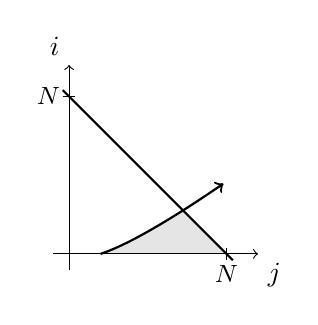
\begin{tikzpicture}[scale = 0.4]
\fill [black!10!white, samples=300, domain=1:3.618] (1,0) --
    plot (\x,{0.5*(1+2*\x-sqrt(1+8*\x))}) -- (5,0) -- cycle;

\draw [->] (-0.5,0) -- (6,0) node [below right] {$j$};
\draw [->] (0,-0.5) -- (0,6) node [above left] {$i$};

\draw [thick] (-0.2,5.2) -- (5.2,-0.2);
\draw [thick, ->, samples=300, domain=1:4.9] plot (\x,{0.5*(1+2*\x-sqrt(1+8*\x))});

\draw (-0.2,5) -- (0.2,5) node [left, xshift = -2pt] {\small $N$};
\draw (5,-0.2) -- (5,0.2) node [below, yshift = -3pt] {\small $N$};
\end{tikzpicture}\qedhere\]
\end{proof}

\end{document}
